% Capítulo 5: Diseño. Fuente de la memoria (D-07): se edita directamente.
% Las figuras salen de generadores/ (gen_seleccion_crm.py, gen_bd_*.py): no se editan a mano.

\chapter{Diseño}\label{sec:dis}

Este capítulo cierra la elección de la plataforma y diseña la base de datos que la sostiene. Primero se describe el proceso de selección del CRM, se compara SuiteCRM con otros productos del mercado y se justifica por qué encaja con un centro de primaria. Después se presenta el diseño de la base de datos en sus tres niveles: conceptual, lógico y físico. Cada nivel parte del anterior y de la especificación del capítulo~\ref{sec:4}, de modo que las restricciones OCL del apartado~\ref{sec:4-2-2} quedan asignadas a un mecanismo concreto en el diseño físico.

% ============================================================================
\needspace{6\baselineskip}
\section{Selección de la plataforma CRM}\label{sec:dis-seleccion}

\needspace{6\baselineskip}
\subsection{Planteamiento del proceso}\label{sec:dis-proceso}

El apartado~\ref{sec:1-2-6} adoptó SuiteCRM como candidata provisional a partir de una comparación documental de tres plataformas. Esa comparación dejaba fuera productos habituales en el mercado y trataba el coste y la licencia como un criterio más, con un peso del 10~\%. Para cerrar la decisión se ha seguido un proceso más amplio, en cinco fases (Figura~\ref{fig:seleccion}):

\begin{enumerate}
  \item \textbf{Lista larga.} Se reúnen nueve CRM de uso extendido, de código abierto y propietarios, incluidas las tres candidatas del apartado~\ref{sec:1-2-4}.
  \item \textbf{Criterio eliminatorio.} Se descartan los productos que no son gratuitos y de código abierto.
  \item \textbf{Lista corta.} Quedan los candidatos que superan el criterio eliminatorio.
  \item \textbf{Matriz ponderada.} Los candidatos de la lista corta se puntúan con seis criterios cuyos pesos se fijan antes de puntuar, para no ajustarlos al resultado. La robustez del resultado se comprueba con un análisis de sensibilidad.
  \item \textbf{Selección.} Se elige la plataforma con mayor puntuación, condicionada a que las pruebas de concepto del apartado~\ref{sec:1-2-5} confirmen las capacidades documentadas.
\end{enumerate}

\begin{figure}[H]
\centering
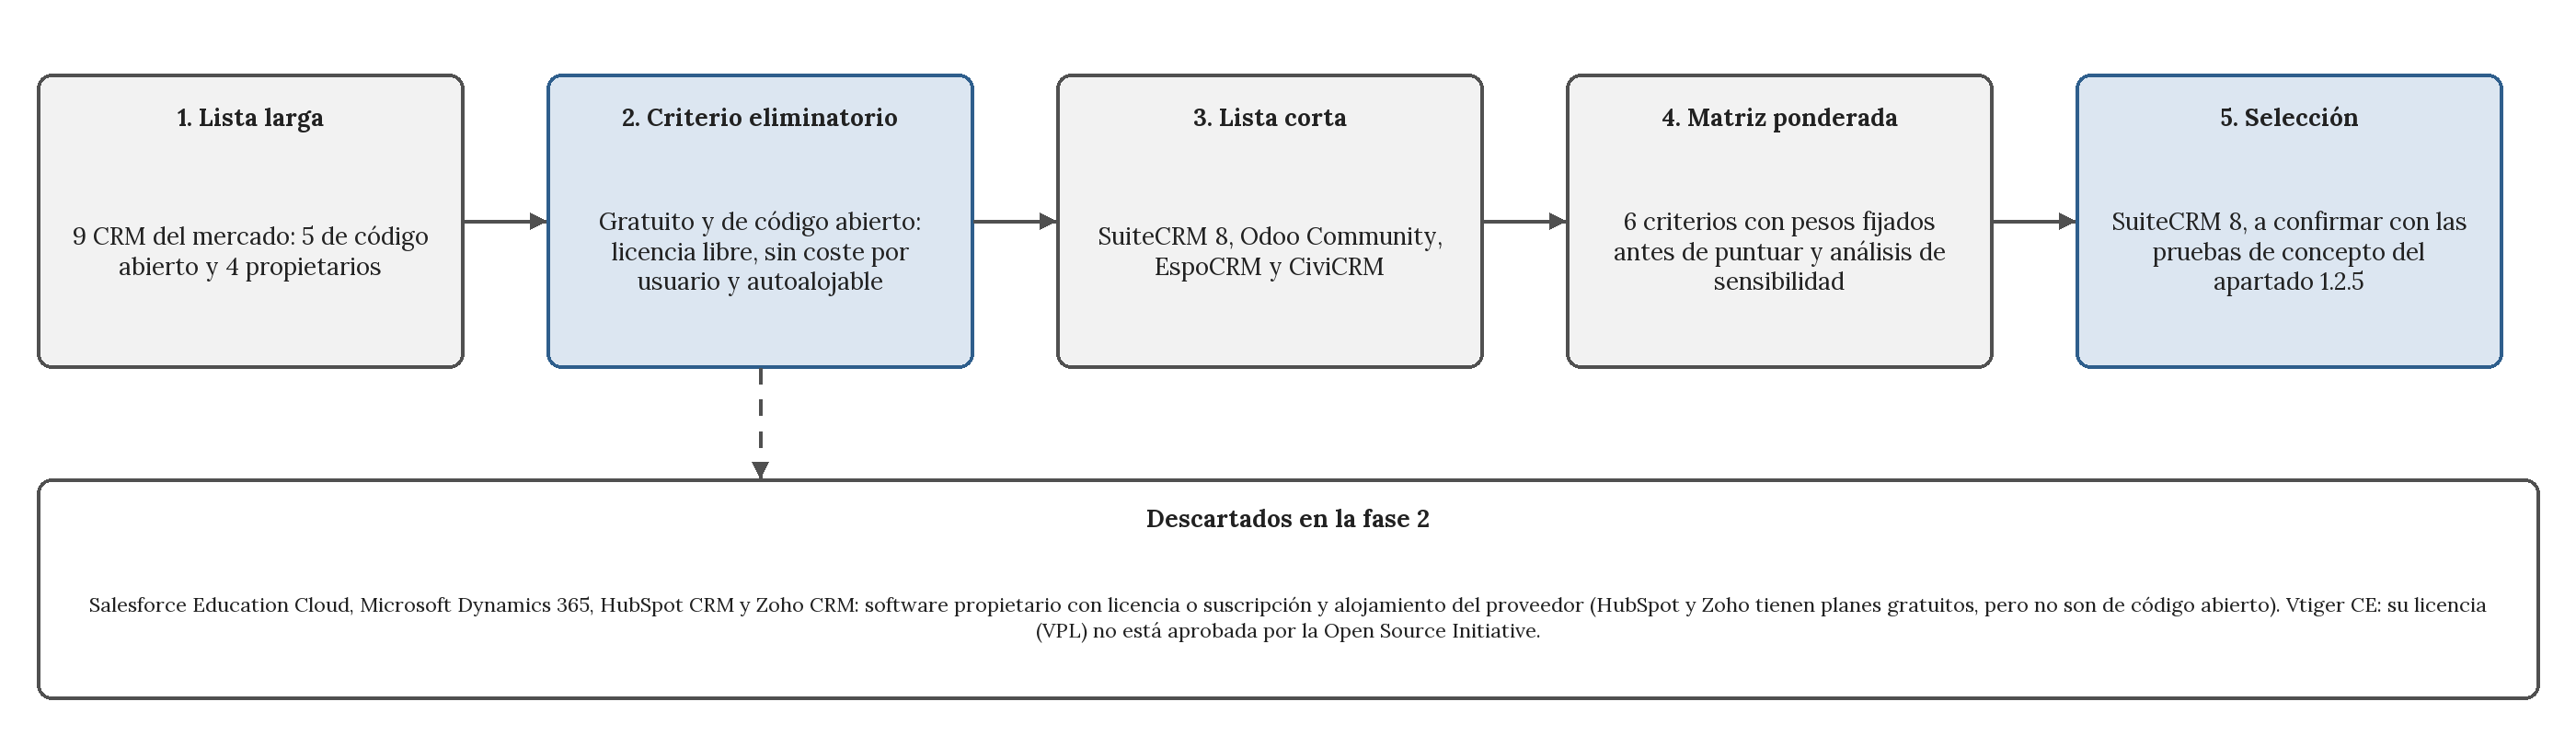
\includegraphics[width=\textwidth]{imagenes/seleccion_crm.png}
\caption[Proceso de selección de la plataforma CRM]{Proceso de selección de la plataforma CRM, desde la lista larga de nueve productos hasta la elección de SuiteCRM 8}\label{fig:seleccion}
\end{figure}

\needspace{6\baselineskip}
\subsection{Candidatos del mercado}\label{sec:dis-candidatos}

La lista larga combina tres grupos. El primero son los CRM de código abierto que se pueden instalar en un servidor propio: SuiteCRM~\cite{ref05,ref06}, Odoo en su edición Community~\cite{ref10,ref48}, EspoCRM~\cite{ref42}, Vtiger CRM en su edición Community~\cite{ref43} y CiviCRM~\cite{ref44}. El segundo son los CRM propietarios con mayor presencia en empresas y en el sector educativo: Salesforce Education Cloud~\cite{ref11} y Microsoft Dynamics~365~\cite{ref47}. El tercero son los CRM propietarios que ofrecen un plan gratuito, HubSpot CRM~\cite{ref46} y Zoho CRM~\cite{ref45}, que podrían parecer adecuados para un centro con poco presupuesto. La Tabla~\ref{tab:dis-candidatos} resume la licencia, el coste y el modelo de alojamiento de cada uno.

\begin{table}[H]
\centering\footnotesize
\begin{tabularx}{\textwidth}{>{\hsize=0.80\hsize\raggedright\arraybackslash}X>{\hsize=1.00\hsize\raggedright\arraybackslash}X>{\hsize=0.95\hsize\raggedright\arraybackslash}X>{\hsize=0.85\hsize\raggedright\arraybackslash}X>{\hsize=1.40\hsize\raggedright\arraybackslash}X}
\toprule
\rowcolor{cabeceratabla} \textbf{CRM} & \textbf{Licencia} & \textbf{Coste de licencia} & \textbf{Alojamiento} & \textbf{Observaciones} \\
\midrule
SuiteCRM 8 & AGPLv3~\cite{ref06} & Ninguno & Servidor propio & Módulos, relaciones, roles, grupos de seguridad y flujos de trabajo configurables~\cite{ref07,ref08,ref09}. \\
Odoo Community & LGPLv3~\cite{ref48} & Ninguno & Servidor propio & Parte de las funciones y aplicaciones solo existe en la edición Enterprise, de pago. \\
EspoCRM & AGPLv3~\cite{ref42} & Ninguno & Servidor propio & El núcleo es gratuito; algunas extensiones oficiales, como los informes y flujos avanzados, se venden aparte. \\
Vtiger CRM (CE) & Vtiger Public License~\cite{ref43} & Ninguno & Servidor propio & Licencia derivada de la MPL que no figura entre las aprobadas por la Open Source Initiative. \\
CiviCRM & AGPLv3 con excepción~\cite{ref44} & Ninguno & Servidor propio, dentro de un CMS & Orientado a entidades sin ánimo de lucro: socios, donaciones y eventos. \\
Salesforce Education Cloud & Propietaria~\cite{ref11} & Suscripción & Nube del proveedor & Modelo de datos educativo amplio (estudiantes y tutores). \\
Microsoft Dynamics 365 & Propietaria~\cite{ref47} & Suscripción & Nube del proveedor & Plataforma empresarial con licencia por usuario. \\
HubSpot CRM & Propietaria~\cite{ref46} & Plan gratuito con límites & Nube del proveedor & Funciones avanzadas en planes de pago. \\
Zoho CRM & Propietaria~\cite{ref45} & Edición gratuita para tres usuarios & Nube del proveedor & Más usuarios o funciones requieren un plan de pago. \\
\bottomrule
\end{tabularx}
\caption{Candidatos de la lista larga}\label{tab:dis-candidatos}
\end{table}

\needspace{6\baselineskip}
\subsection{Criterio eliminatorio: gratuito y de código abierto}\label{sec:dis-eliminatorio}

El primer filtro exige que la plataforma sea gratuita y de código abierto. Se considera que un producto cumple el criterio cuando se dan tres condiciones a la vez: su licencia es libre según la definición de la Open Source Initiative~\cite{ref49}, su uso no exige pagar licencias por usuario y se puede instalar en una infraestructura que controle el centro o su proveedor. El criterio es eliminatorio por cuatro motivos que salen del propio proyecto:

\begin{itemize}
  \item \textbf{Coste.} Un centro de primaria, o la asociación de familias que organiza las extraescolares, no suele disponer de presupuesto para suscripciones por usuario. El presupuesto del apartado~\ref{sec:3-1-1} ya parte de usar software sin coste de licencia.
  \item \textbf{Control de los datos.} El sistema guarda datos de menores (RNF02). Con un producto autoalojado, el centro decide dónde residen los datos, quién los administra y cómo se hacen y se conservan las copias, tal como piden el RGPD y la AEPD~\cite{ref02,ref03,ref04}.
  \item \textbf{Objetivo del TFG.} El trabajo consiste en estudiar y adaptar un CRM. Con el código disponible se puede comprobar cómo se aplican los permisos o la auditoría, en lugar de depender de lo que diga la documentación comercial.
  \item \textbf{Dependencia del proveedor.} Un producto libre se puede mantener aunque cambien las condiciones del fabricante, y la información se puede exportar sin restricciones (RNF05).
\end{itemize}

Con este criterio quedan fuera los cuatro productos propietarios. Entre ellos está Salesforce Education Cloud, que en la evaluación provisional (Tabla~\ref{tab:3}) quedaba tercera precisamente por su coste y su dependencia del proveedor. HubSpot CRM y Zoho CRM ofrecen planes gratuitos, pero su código no es abierto, los datos se alojan en la nube del proveedor y los límites del plan gratuito los fija el fabricante~\cite{ref45,ref46}. Vtiger CRM se distribuye como código abierto, pero su licencia no figura entre las aprobadas por la Open Source Initiative~\cite{ref43}, así que tampoco cumple la primera condición. La lista corta queda formada por SuiteCRM~8, Odoo Community, EspoCRM y CiviCRM.

\needspace{6\baselineskip}
\subsection{Criterios y pesos de la evaluación}\label{sec:dis-criterios}

Los candidatos de la lista corta se comparan con los criterios de la Tabla~\ref{tab:dis-criterios}. Respecto a la matriz provisional (Tabla~\ref{tab:2}) hay dos cambios. El criterio de coste y licencia desaparece de la matriz porque ya actúa como filtro eliminatorio y todos los candidatos que quedan lo cumplen. En su lugar entra la comunidad y la documentación, que mide si existe ayuda suficiente para mantener la solución cuando el proyecto termine.

\begin{table}[H]
\centering\small
\begin{tabularx}{\textwidth}{>{\hsize=0.70\hsize\raggedright\arraybackslash}X>{\hsize=0.30\hsize\raggedright\arraybackslash}X>{\hsize=2.00\hsize\raggedright\arraybackslash}X}
\toprule
\rowcolor{cabeceratabla} \textbf{Criterio} & \textbf{Peso} & \textbf{Qué se evalúa} \\
\midrule
Adecuación funcional & 25 \% & Cobertura nativa o configurable de personas, relaciones, sesiones, estados y comunicaciones (RF01--RF07). \\
Privacidad y seguridad & 20 \% & Roles, permisos a nivel de registro, auditoría de cambios y autenticación (RNF01, RNF02). \\
Extensibilidad & 20 \% & Creación de entidades y relaciones propias, reglas, API y extensiones que no modifican el núcleo (RNF05). \\
Control de despliegue y datos & 15 \% & Instalación propia, copias, exportación y portabilidad (RNF04). \\
Usabilidad y aprendizaje & 10 \% & Interfaz web adaptable, coherencia y esfuerzo de formación de monitores y coordinación (RNF06). \\
Comunidad y documentación & 10 \% & Documentación oficial, actividad del proyecto y ayuda disponible para el mantenimiento. \\
\bottomrule
\end{tabularx}
\caption{Criterios y pesos de la matriz de selección}\label{tab:dis-criterios}
\end{table}

Cada criterio se puntúa de 1 a 5 con la misma escala del apartado~\ref{sec:1-2-5}: 1 si el candidato no cubre la necesidad o exige una solución externa sustancial, 3 si la cubre de forma parcial con configuración o desarrollo asumible, y 5 si la cubre de forma sólida, verificable y sostenible. La puntuación total es la suma de cada nota multiplicada por su peso.

\needspace{6\baselineskip}
\subsection{Evaluación de la lista corta}\label{sec:dis-evaluacion}

\textbf{SuiteCRM 8.} No incluye objetos escolares, así que alumnos, sesiones o entregas se tienen que crear como módulos nuevos (adecuación funcional, 3). A cambio, Module Builder y Studio permiten crear esos módulos, sus campos y sus relaciones sin tocar el núcleo~\cite{ref07}, y los logic hooks permiten añadir validaciones en el momento de guardar~\cite{ref50} (extensibilidad, 5). Los roles y los grupos de seguridad restringen el acceso por registro, y la auditoría de campos guarda el valor anterior, el nuevo, el autor y la fecha de cada cambio~\cite{ref08} (privacidad y seguridad, 4). Se instala en un servidor propio con una base de datos MySQL o MariaDB (control de despliegue, 5). La interfaz exige algo de formación para usuarios sin experiencia en CRM (usabilidad, 3), y la documentación oficial cubre la administración y el desarrollo de extensiones (comunidad y documentación, 4).

\textbf{Odoo Community.} Odoo tiene un ecosistema de módulos muy amplio y un modelo de permisos con reglas de registro~\cite{ref10} (privacidad y seguridad, 4). Su módulo de asistencia está pensado para empleados, por lo que habría que adaptarlo para el alumnado (adecuación, 3). Las extensiones se escriben como módulos en Python, lo que da mucho control pero obliga a programar incluso cambios sencillos, porque la herramienta de personalización visual pertenece a la edición Enterprise (extensibilidad, 4). La evaluación provisional le daba un 5 en este criterio sin distinguir entre ediciones; al limitar la comparación a lo gratuito, la nota baja. Parte de las aplicaciones también es exclusiva de Enterprise~\cite{ref48}, lo que limita lo que se puede usar sin coste (control de despliegue, 4). Su interfaz es moderna (usabilidad, 4) y tiene una comunidad grande (comunidad, 4).

\textbf{EspoCRM.} Permite definir entidades y relaciones propias desde la administración y controla el acceso por rol con niveles de propiedad del registro (adecuación, 3; privacidad y seguridad, 4). Su interfaz es ligera y fácil de aprender (usabilidad, 4) y se autoaloja sin coste~\cite{ref42} (control de despliegue, 5). Los informes y los flujos de trabajo avanzados se distribuyen como extensión de pago, y en un centro sin presupuesto eso deja fuera los avisos y escalados automáticos (extensibilidad, 4). Su comunidad es más pequeña que la de SuiteCRM u Odoo (comunidad, 3).

\textbf{CiviCRM.} Está diseñado para entidades sin ánimo de lucro: gestiona socios, eventos y donaciones, y los eventos con participantes podrían representar en parte las sesiones (adecuación, 3). Se instala dentro de un gestor de contenidos (Drupal, WordPress, Joomla o Backdrop), y los permisos se reparten entre CiviCRM y ese gestor, lo que complica restringir un monitor a sus grupos (privacidad y seguridad, 3). Tiene API y sistema de extensiones (extensibilidad, 4) y se autoaloja sin coste~\cite{ref44} (control de despliegue, 5). La dependencia del gestor de contenidos aumenta el esfuerzo de instalación y de formación (usabilidad, 2). Tiene una comunidad activa en el sector no lucrativo (comunidad, 4).

La Tabla~\ref{tab:dis-matriz} reúne las puntuaciones.

\begin{table}[H]
\centering\small
\begin{tabularx}{\textwidth}{>{\hsize=1.55\hsize\raggedright\arraybackslash}X>{\hsize=0.55\hsize\raggedright\arraybackslash}X>{\hsize=0.95\hsize\raggedright\arraybackslash}X>{\hsize=0.95\hsize\raggedright\arraybackslash}X>{\hsize=0.95\hsize\raggedright\arraybackslash}X>{\hsize=1.05\hsize\raggedright\arraybackslash}X}
\toprule
\rowcolor{cabeceratabla} \textbf{Criterio} & \textbf{Peso} & \textbf{SuiteCRM 8} & \textbf{Odoo Community} & \textbf{EspoCRM} & \textbf{CiviCRM} \\
\midrule
Adecuación funcional & 25 \% & 3 & 3 & 3 & 3 \\
Privacidad y seguridad & 20 \% & 4 & 4 & 4 & 3 \\
Extensibilidad & 20 \% & 5 & 4 & 4 & 4 \\
Control de despliegue y datos & 15 \% & 5 & 4 & 5 & 5 \\
Usabilidad y aprendizaje & 10 \% & 3 & 4 & 4 & 2 \\
Comunidad y documentación & 10 \% & 4 & 4 & 3 & 4 \\
\midrule
\textbf{Resultado ponderado} & 100 \% & \textbf{4,00} & 3,75 & 3,80 & 3,50 \\
Media sin ponderar & -- & 4,00 & 3,83 & 3,83 & 3,50 \\
\bottomrule
\end{tabularx}
\caption{Matriz ponderada de la lista corta}\label{tab:dis-matriz}
\end{table}

SuiteCRM obtiene la mayor puntuación (4,00), seguido de EspoCRM (3,80), Odoo Community (3,75) y CiviCRM (3,50). La ventaja de SuiteCRM procede de la extensibilidad y del control del despliegue: es el único candidato que permite crear las entidades del proyecto, sus relaciones, sus validaciones y sus flujos de trabajo sin coste adicional y sin modificar el núcleo.

Para comprobar que el resultado no depende de los pesos elegidos se han hecho dos pruebas de sensibilidad. Con todos los criterios al mismo peso (última fila de la Tabla~\ref{tab:dis-matriz}), SuiteCRM sigue primero, con 4,00 frente a 3,83 de EspoCRM y Odoo. Si se duplica el peso de la usabilidad, que es el criterio más desfavorable para SuiteCRM, y se reparte el exceso entre los demás de forma proporcional, la puntuación de SuiteCRM baja a 3,89 y la de EspoCRM sube a 3,82, así que el orden se mantiene. Comparando las notas criterio a criterio, EspoCRM solo pasaría delante si la usabilidad pesara más que la extensibilidad y la comunidad juntas, y Odoo, si pesara más que la extensibilidad y el control del despliegue juntos. Ninguno de los dos repartos tiene sentido en un proyecto que consiste en adaptar la plataforma.

Las puntuaciones tienen una limitación: se basan en la documentación oficial de cada producto. Por eso la decisión queda condicionada a las pruebas de concepto descritas en el apartado~\ref{sec:1-2-5}. Si alguna contradice una capacidad documentada, se corrige la nota y se recalcula la matriz.

\needspace{6\baselineskip}
\subsection{Adecuación de SuiteCRM al proyecto}\label{sec:dis-adecuacion}

La Tabla~\ref{tab:dis-adecuacion} relaciona cada necesidad del proyecto con la capacidad de SuiteCRM que la cubre y con la forma en que se usará en el prototipo.

\begin{table}[H]
\centering\footnotesize
\begin{tabularx}{\textwidth}{>{\hsize=0.85\hsize\raggedright\arraybackslash}X>{\hsize=1.05\hsize\raggedright\arraybackslash}X>{\hsize=1.10\hsize\raggedright\arraybackslash}X}
\toprule
\rowcolor{cabeceratabla} \textbf{Necesidad} & \textbf{Capacidad de SuiteCRM} & \textbf{Uso en el prototipo} \\
\midrule
Entidades escolares (RF01--RF06) & Module Builder y Studio~\cite{ref07} & Módulos \texttt{ext\_*} para alumnos, autorizaciones, actividades, grupos, inscripciones, sesiones, asistencias, entregas, incidencias, actuaciones y comunicaciones. \\
Personas autorizadas & Módulo Contactos del núcleo & Las personas autorizadas son contactos, con un campo adicional para la relación con el alumno. \\
Acceso por grupo (RF07, RNF01) & Roles y grupos de seguridad~\cite{ref08} & Cada monitor solo ve los registros de los grupos que tiene asignados. \\
Trazabilidad de cambios (RF03, R07) & Auditoría de campos & Las correcciones de asistencia, autorizaciones, entregas e incidencias guardan el valor anterior, el nuevo, el autor y la fecha. \\
Reglas de integridad (OCL) & Logic hooks~\cite{ref50} & Validaciones antes de guardar para las reglas que implican varias tablas (OCL02, OCL05, OCL08). \\
Avisos y escalados (RF05, RF06) & Workflows~\cite{ref09} & Tareas de verificación ante una ausencia y avisos a coordinación ante una entrega bloqueada. \\
Datos de menores (RNF02) & Instalación propia, licencia AGPLv3~\cite{ref06} & El centro decide dónde se alojan los datos y quién los administra; sin coste de licencia. \\
Mantenimiento (RNF05) & Extensiones en \texttt{custom/} y paquetes instalables & El paquete «Gestión de Extraescolares» se versiona en el repositorio y no modifica el núcleo. \\
\bottomrule
\end{tabularx}
\caption{Adecuación de SuiteCRM a las necesidades del proyecto}\label{tab:dis-adecuacion}
\end{table}

La elección también tiene inconvenientes que el diseño tiene en cuenta. SuiteCRM no trae ningún objeto escolar, así que todo el modelo de datos de los apartados siguientes es trabajo propio. Su interfaz está pensada para usuarios de oficina, y el registro de asistencia y entrega en tres acciones (RNF06) obliga a preparar vistas simplificadas para los monitores. La licencia AGPLv3 obliga a publicar el código de las modificaciones si se ofrecen a terceros a través de la red~\cite{ref06}; en un proyecto académico con el repositorio público esto no supone ninguna restricción.

% ============================================================================
\needspace{6\baselineskip}
\section{Diseño conceptual de la base de datos}\label{sec:dis-conceptual}

El diseño conceptual describe qué información guarda el sistema, con independencia de la plataforma. Parte del modelo conceptual de la especificación (apartado~\ref{sec:4-2}) y lo completa con las entidades que allí quedaban implícitas: la inscripción, la actividad, el grupo, la persona autorizada, la actuación sobre una incidencia y el usuario. La Figura~\ref{fig:bd-conceptual} lo representa como un diagrama de clases UML~\cite{ref35,ref51}.

\begin{sidewaysfigure}
\centering
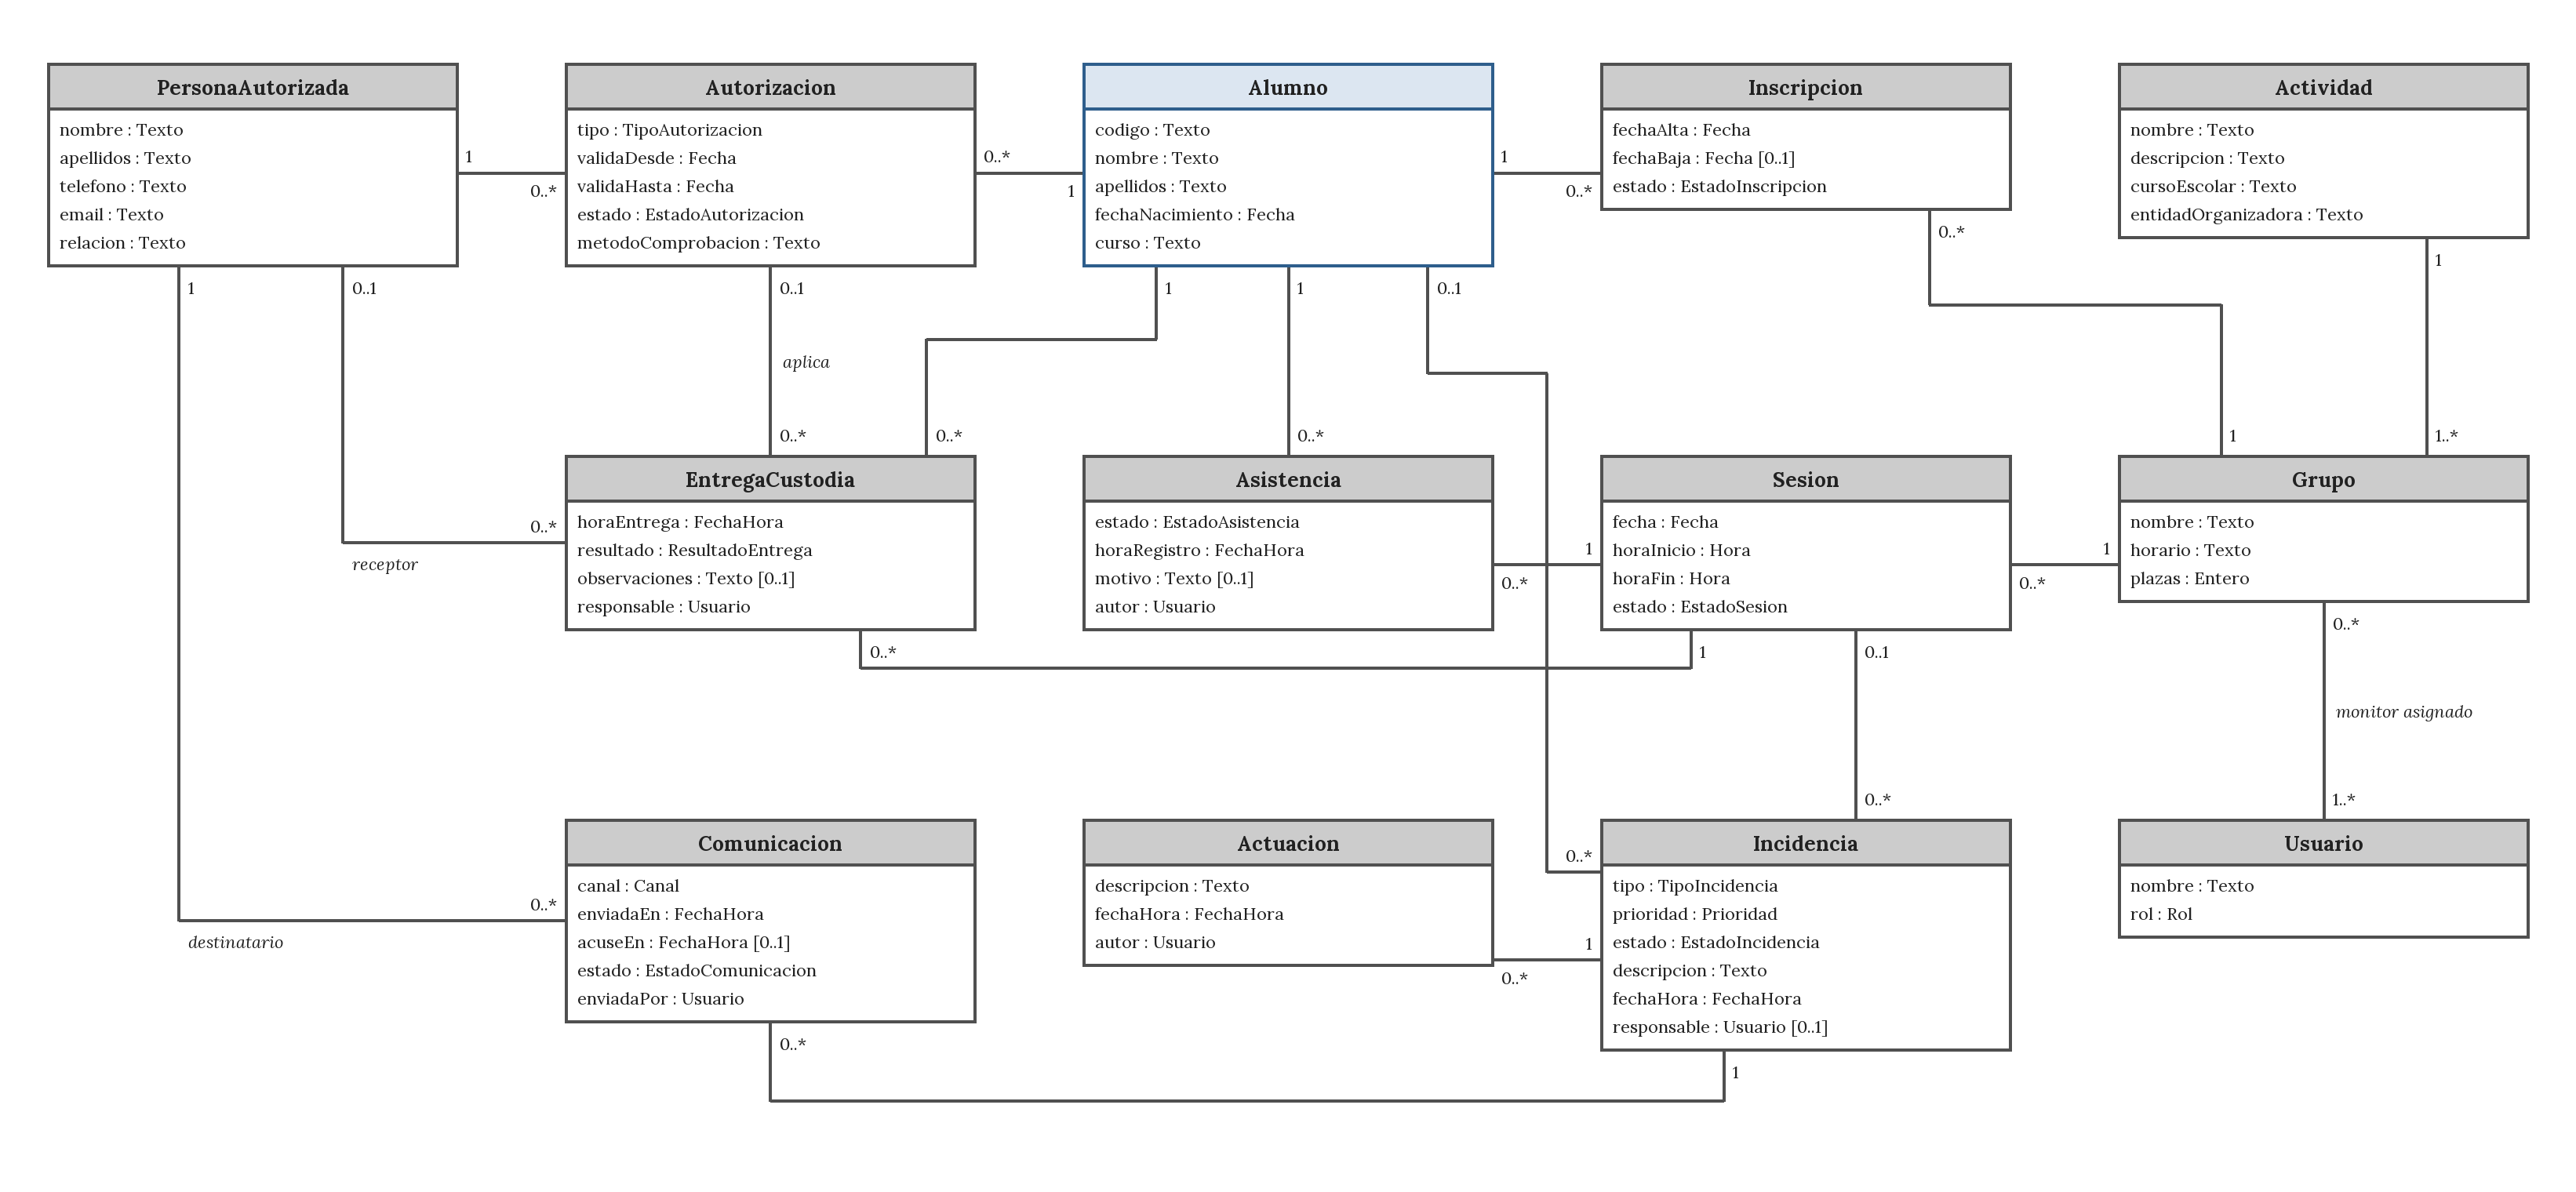
\includegraphics[width=\textheight,height=0.92\textwidth,keepaspectratio]{imagenes/bd_conceptual.png}
\caption[Diseño conceptual de la base de datos]{Diseño conceptual de la base de datos (diagrama de clases UML). Los atributos de tipo Usuario indican quién registra un hecho o es responsable de él}\label{fig:bd-conceptual}
\end{sidewaysfigure}

El alumno es la entidad central. A su alrededor se organizan tres grupos de información:

\begin{itemize}
  \item \textbf{Organización de las actividades.} Una actividad tiene uno o más grupos, cada grupo tiene sesiones y uno o más monitores asignados, y la inscripción vincula a un alumno con un grupo durante un periodo.
  \item \textbf{Custodia.} Una autorización vincula a un alumno con una persona autorizada durante un periodo de vigencia. Cada entrega registra el alumno, la sesión, la persona que lo recoge y la autorización aplicada.
  \item \textbf{Seguimiento.} La asistencia registra el estado de cada alumno en cada sesión. Una incidencia puede referirse a un alumno, a una sesión o a ambos, y acumula las actuaciones realizadas y las comunicaciones enviadas.
\end{itemize}

En este nivel se han tomado tres decisiones de diseño:

\begin{enumerate}
  \item \textbf{La inscripción se hace en un grupo y no en la actividad.} Una actividad puede tener varios grupos con horarios y monitores distintos, y la lista de una sesión tiene que contener solo los alumnos de su grupo. La actividad se obtiene a través del grupo, así que la lista por actividad sigue siendo posible. Esta decisión resuelve la diferencia entre la memoria (apartado~\ref{sec:1-2-7}) y el caso de uso CU02, que hablaba de inscripciones de la actividad.
  \item \textbf{Las correcciones de asistencia se guardan en la auditoría.} Cada alumno tiene un único registro de asistencia por sesión (OCL03), y cada cambio de estado o de motivo queda en la tabla de auditoría con el valor anterior, el nuevo, el autor y la fecha. Así se cumplen a la vez la restricción de unicidad y la regla R07, que pide no perder el historial.
  \item \textbf{La vigencia de una autorización se calcula y no se guarda.} El estado guardado solo distingue entre activa y revocada. Que una autorización esté vencida se deduce de sus fechas en el momento de la entrega, lo que evita tener que actualizar estados cada día.
\end{enumerate}

Las enumeraciones del diagrama toman los valores de la Tabla~\ref{tab:dis-enumeraciones}.

\begin{table}[H]
\centering\small
\begin{tabularx}{\textwidth}{>{\hsize=0.65\hsize\raggedright\arraybackslash}X>{\hsize=1.35\hsize\raggedright\arraybackslash}X}
\toprule
\rowcolor{cabeceratabla} \textbf{Enumeración} & \textbf{Valores} \\
\midrule
TipoAutorizacion & responsable legal, recogida \\
EstadoAutorizacion & activa, revocada (la vigencia se calcula con las fechas) \\
EstadoInscripcion & activa, cancelada \\
EstadoSesion & programada, publicada, cerrada \\
EstadoAsistencia & presente, ausente, retraso, ausencia justificada \\
ResultadoEntrega & confirmada, bloqueada, escalada \\
TipoIncidencia & salud, conducta, accidente, recogida, otra \\
Prioridad & baja, media, alta \\
EstadoIncidencia & abierta, en curso, escalada, cerrada \\
Canal & correo electrónico, teléfono, presencial \\
EstadoComunicacion & preparada, enviada, con acuse \\
Rol & administración, coordinación, monitor, dirección \\
\bottomrule
\end{tabularx}
\caption{Valores de las enumeraciones del modelo conceptual}\label{tab:dis-enumeraciones}
\end{table}

% ============================================================================
\needspace{6\baselineskip}
\section{Diseño lógico de la base de datos}\label{sec:dis-logico}

El diseño lógico traduce el modelo conceptual a un esquema relacional~\cite{ref51} y lo adapta a las convenciones de SuiteCRM. Se han aplicado estas reglas de transformación:

\begin{itemize}
  \item Cada entidad se convierte en una tabla con una clave primaria \texttt{id}, un identificador universal (UUID) de 36 caracteres, que es el formato que usa SuiteCRM.
  \item Cada asociación de uno a muchos se convierte en una clave ajena en la tabla del lado «muchos». Las asociaciones opcionales (multiplicidad 0..1) admiten el valor nulo.
  \item La asociación de muchos a muchos entre grupos y monitores se convierte en la tabla de relación \texttt{ext\_grupos\_users}.
  \item La autorización, que en el modelo conceptual une alumno y persona autorizada con sus propios atributos, se convierte en la tabla \texttt{ext\_autorizaciones} con una clave ajena hacia cada lado.
  \item Las entidades que ya existen en SuiteCRM se reutilizan: las personas autorizadas son contactos (\texttt{contacts}, con el campo propio \texttt{relacion\_c} en \texttt{contacts\_cstm}) y los usuarios son los de la plataforma (\texttt{users}), con sus roles y grupos de seguridad.
  \item Las tablas nuevas llevan el prefijo \texttt{ext\_} para distinguirlas del núcleo. Además de las columnas de la figura, cada una tiene los campos comunes de SuiteCRM: \texttt{date\_entered}, \texttt{date\_modified}, \texttt{created\_by}, \texttt{modified\_user\_id} y \texttt{deleted}, que implementa el borrado lógico.
\end{itemize}

La Figura~\ref{fig:bd-logico} muestra el esquema resultante y la Tabla~\ref{tab:dis-esquema} lo resume.

\begin{sidewaysfigure}
\centering
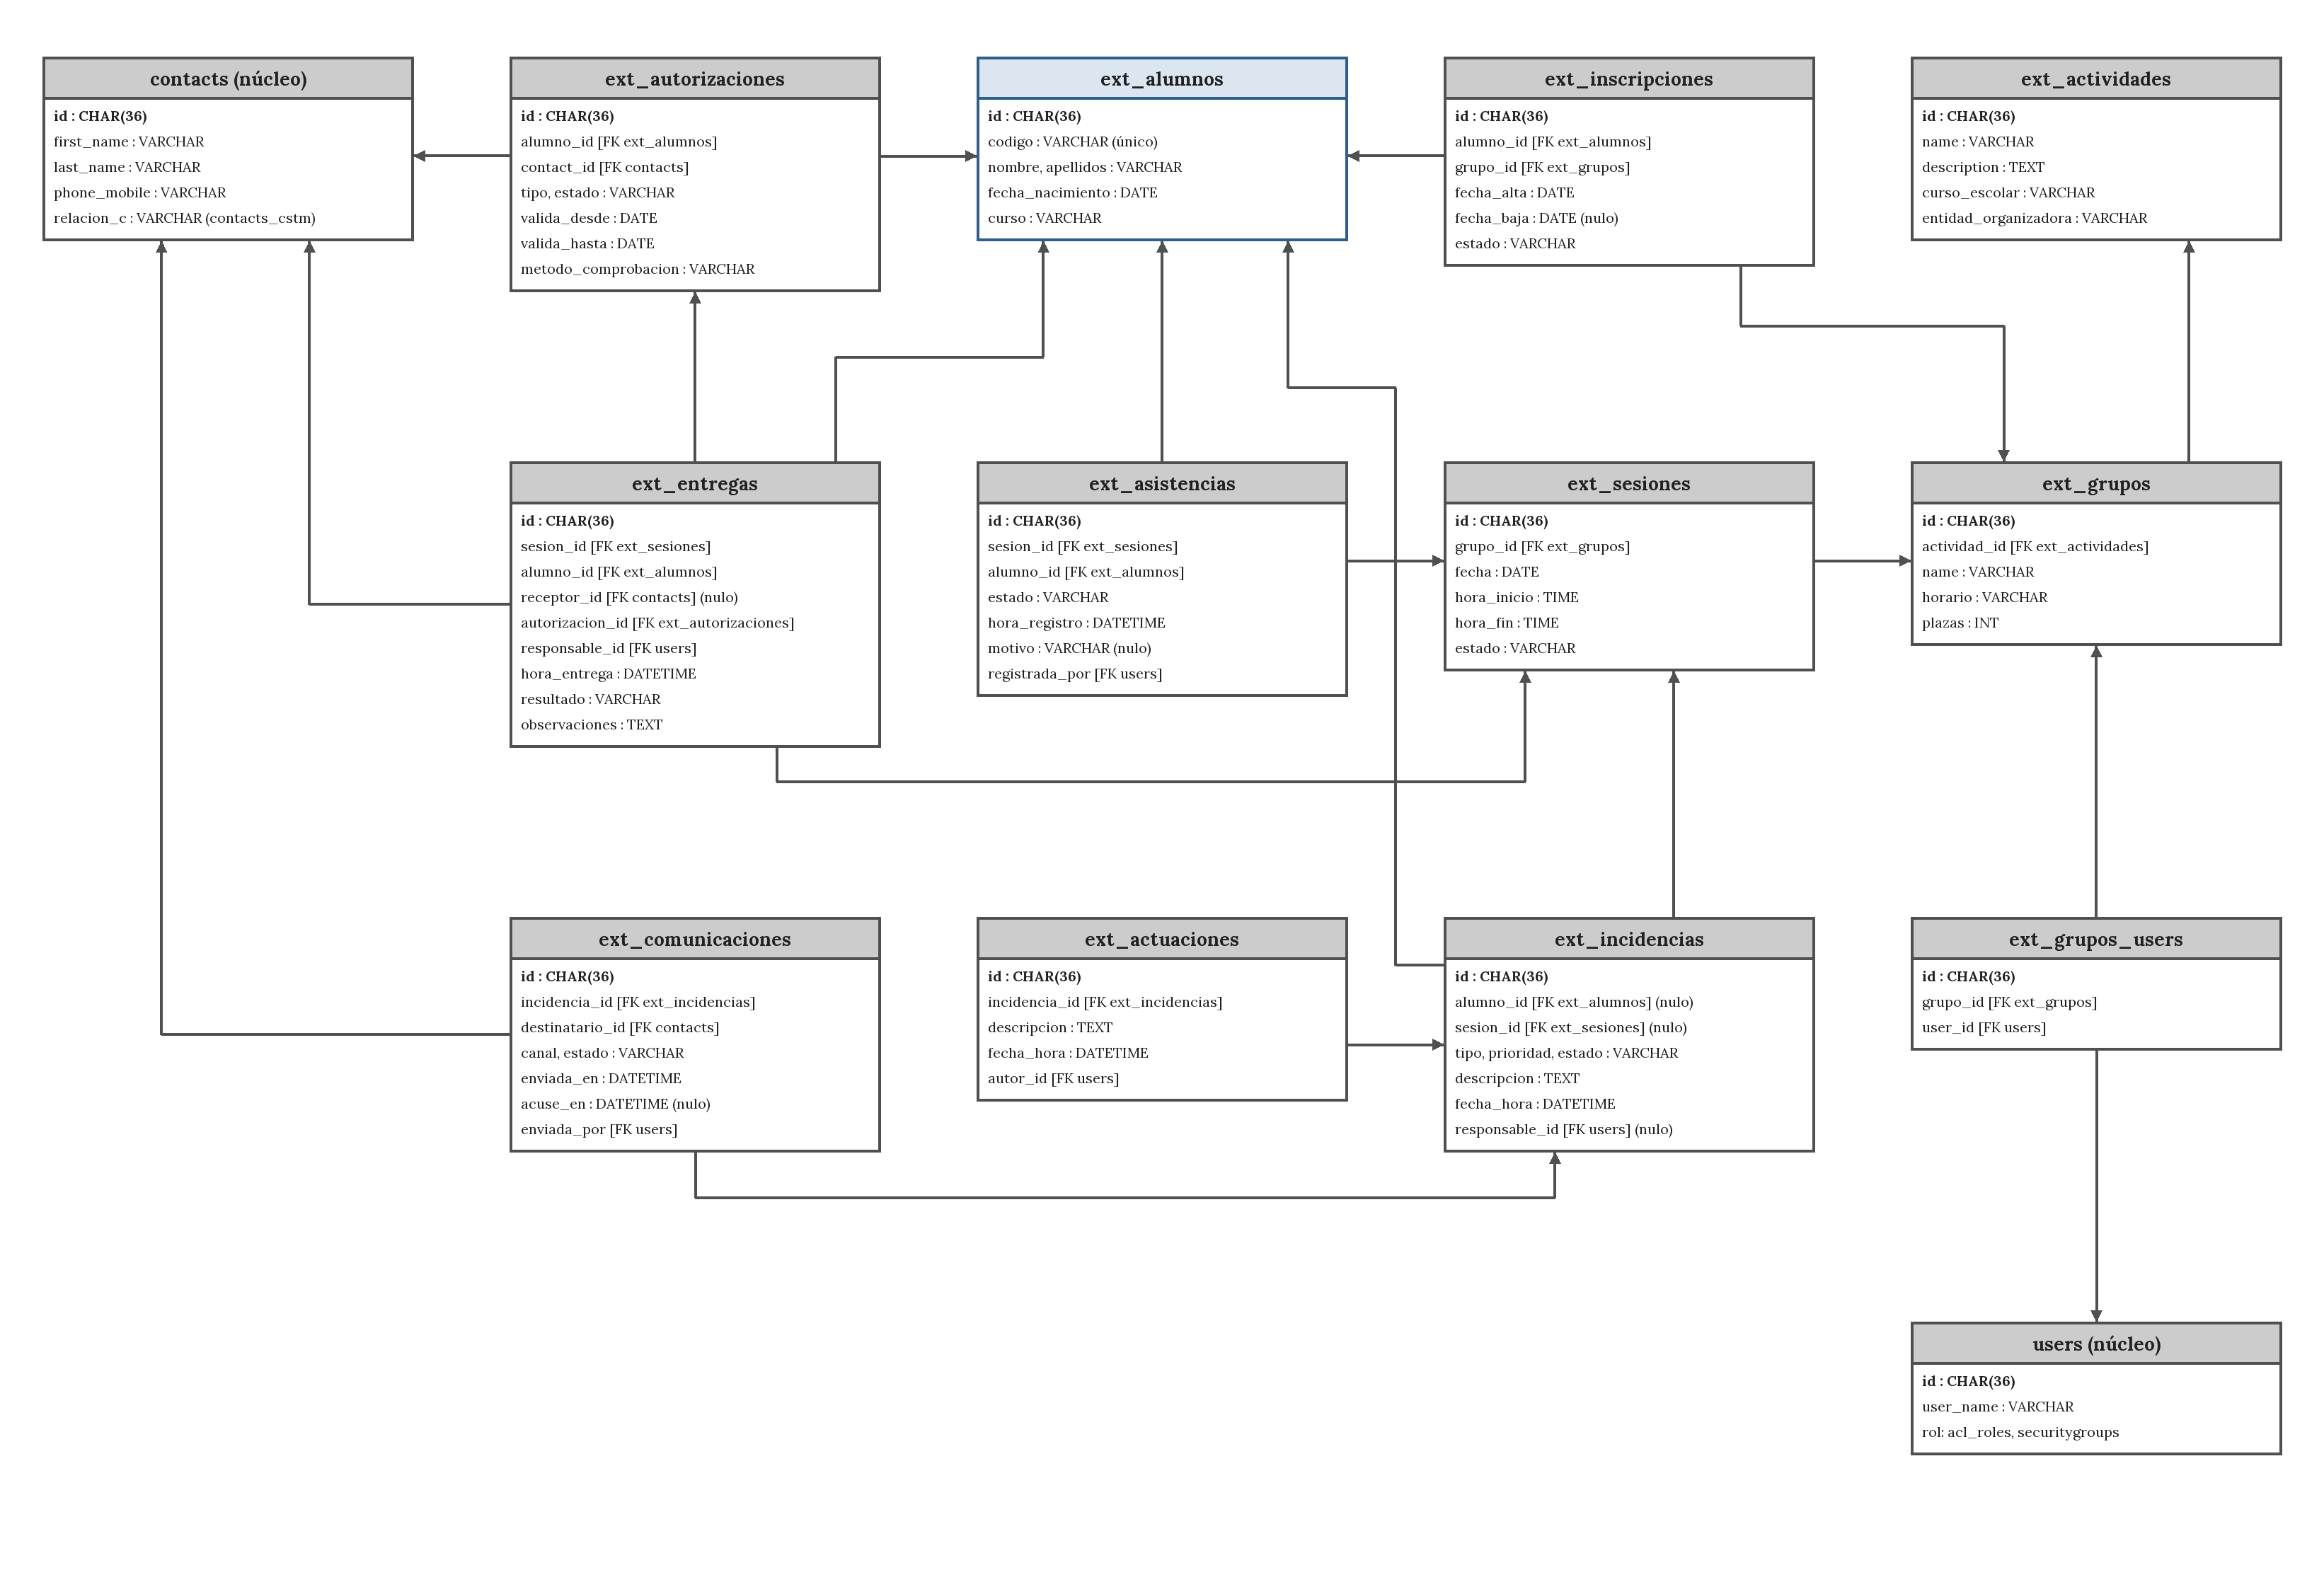
\includegraphics[width=\textheight,height=0.92\textwidth,keepaspectratio]{imagenes/bd_logico.png}
\caption[Diseño lógico de la base de datos]{Diseño lógico de la base de datos (esquema relacional). La clave primaria va en negrita y cada flecha va de una clave ajena a la tabla que referencia; las claves ajenas hacia \texttt{users} se indican en la columna y no se dibujan}\label{fig:bd-logico}
\end{sidewaysfigure}

\begin{table}[H]
\centering\footnotesize
\begin{tabularx}{\textwidth}{>{\hsize=0.85\hsize\raggedright\arraybackslash}X>{\hsize=1.35\hsize\raggedright\arraybackslash}X>{\hsize=0.80\hsize\raggedright\arraybackslash}X}
\toprule
\rowcolor{cabeceratabla} \textbf{Tabla} & \textbf{Claves ajenas} & \textbf{Otras restricciones} \\
\midrule
\texttt{ext\_alumnos} & -- & \texttt{codigo} único \\
\texttt{ext\_autorizaciones} & \texttt{alumno\_id}, \texttt{contact\_id} & \texttt{valida\_desde} $\leq$ \texttt{valida\_hasta} (OCL01) \\
\texttt{ext\_actividades} & -- & -- \\
\texttt{ext\_grupos} & \texttt{actividad\_id} & \texttt{plazas} $>$ 0 \\
\texttt{ext\_grupos\_users} & \texttt{grupo\_id}, \texttt{user\_id} & Par (\texttt{grupo\_id}, \texttt{user\_id}) único \\
\texttt{ext\_inscripciones} & \texttt{alumno\_id}, \texttt{grupo\_id} & Una inscripción activa por alumno y grupo \\
\texttt{ext\_sesiones} & \texttt{grupo\_id} & \texttt{hora\_inicio} $<$ \texttt{hora\_fin} (OCL07) \\
\texttt{ext\_asistencias} & \texttt{sesion\_id}, \texttt{alumno\_id}, \texttt{registrada\_por} & Par (\texttt{alumno\_id}, \texttt{sesion\_id}) único (OCL03) \\
\texttt{ext\_entregas} & \texttt{sesion\_id}, \texttt{alumno\_id}, \texttt{receptor\_id}, \texttt{autorizacion\_id}, \texttt{responsable\_id} & Una entrega confirmada por alumno y sesión (OCL04) \\
\texttt{ext\_incidencias} & \texttt{alumno\_id}, \texttt{sesion\_id}, \texttt{responsable\_id} (todas opcionales) & -- \\
\texttt{ext\_actuaciones} & \texttt{incidencia\_id}, \texttt{autor\_id} & -- \\
\texttt{ext\_comunicaciones} & \texttt{incidencia\_id}, \texttt{destinatario\_id}, \texttt{enviada\_por} & -- \\
\bottomrule
\end{tabularx}
\caption{Resumen del esquema relacional}\label{tab:dis-esquema}
\end{table}

El esquema está en tercera forma normal~\cite{ref51}. Todas las tablas tienen una clave primaria simple, los atributos son atómicos y ningún atributo no clave depende de otro atributo no clave. Por ejemplo, el nombre de la actividad no se repite en cada grupo ni en cada sesión: se obtiene siguiendo las claves ajenas \texttt{grupo\_id} y \texttt{actividad\_id}. La única excepción deliberada son los estados de las tablas, que se guardan como texto con valores cerrados (Tabla~\ref{tab:dis-enumeraciones}) porque así es como SuiteCRM almacena las listas desplegables.

% ============================================================================
\needspace{6\baselineskip}
\section{Diseño físico de la base de datos}\label{sec:dis-fisico}

El diseño físico fija cómo se almacena el esquema lógico en el sistema gestor y cómo se hacen cumplir las restricciones. La Figura~\ref{fig:bd-fisico} muestra la organización del almacenamiento y su relación con la aplicación.

\begin{sidewaysfigure}
\centering
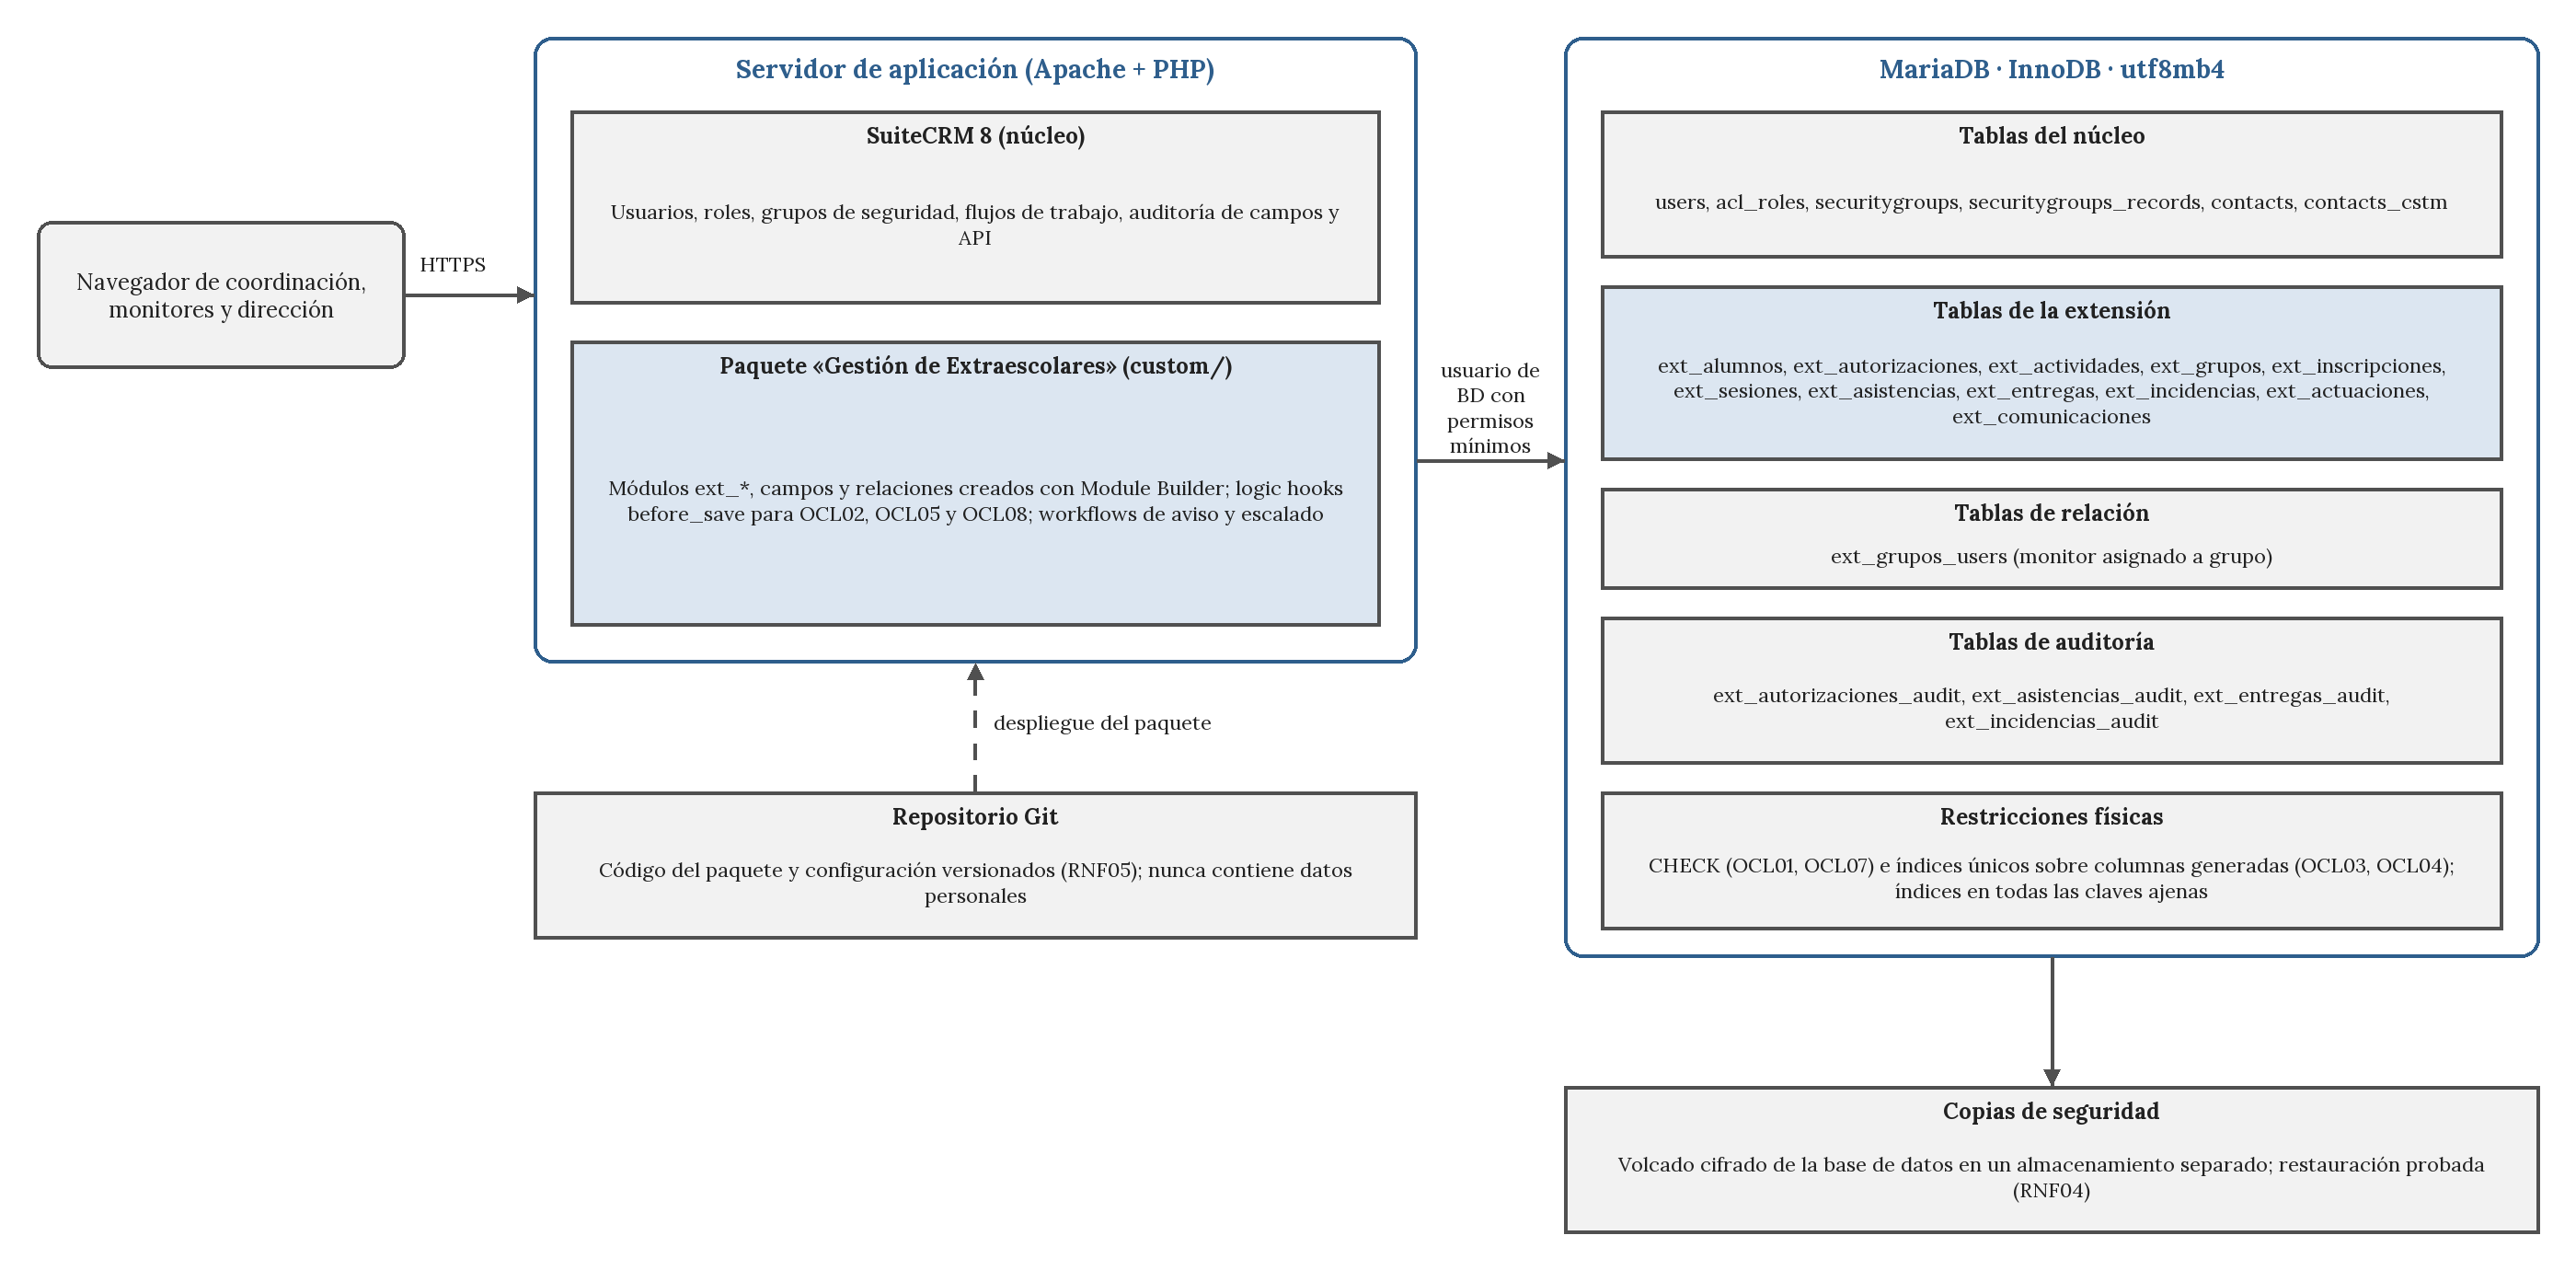
\includegraphics[width=\textheight,height=0.92\textwidth,keepaspectratio]{imagenes/bd_fisico.png}
\caption[Diseño físico del almacenamiento]{Diseño físico del almacenamiento: servidor de aplicación con SuiteCRM y el paquete de extensión, base de datos MariaDB, copias de seguridad y repositorio}\label{fig:bd-fisico}
\end{sidewaysfigure}

\needspace{6\baselineskip}
\subsection{Sistema gestor y tipos de datos}\label{sec:dis-sgbd}

La base de datos es MariaDB, uno de los sistemas gestores que admite SuiteCRM, con el motor InnoDB y el juego de caracteres \texttt{utf8mb4}. InnoDB aporta transacciones y bloqueo por fila, de modo que dos monitores pueden registrar a la vez la asistencia de sesiones distintas sin bloquearse, y \texttt{utf8mb4} guarda correctamente nombres con cualquier carácter. Los tipos de datos siguen las convenciones de SuiteCRM (Tabla~\ref{tab:dis-tipos}). Las fechas y horas se guardan en UTC y la aplicación las convierte a la zona horaria de cada usuario.

\begin{table}[H]
\centering\small
\begin{tabularx}{\textwidth}{>{\hsize=0.85\hsize\raggedright\arraybackslash}X>{\hsize=0.70\hsize\raggedright\arraybackslash}X>{\hsize=1.45\hsize\raggedright\arraybackslash}X}
\toprule
\rowcolor{cabeceratabla} \textbf{Dato} & \textbf{Tipo físico} & \textbf{Motivo} \\
\midrule
Identificadores y claves ajenas & \texttt{CHAR(36)} & UUID generado por SuiteCRM; evita colisiones al importar datos. \\
Nombres, códigos y estados & \texttt{VARCHAR(n)} & Longitud variable; los estados guardan la clave de la lista desplegable. \\
Descripciones y observaciones & \texttt{TEXT} & Texto libre sin longitud fija. \\
Fechas (nacimiento, vigencia, sesión) & \texttt{DATE} & Sin componente horaria. \\
Horas de inicio y fin de sesión & \texttt{TIME} & Solo la hora del día. \\
Momentos de registro y envío & \texttt{DATETIME} (UTC) & Orden temporal exacto para reconstruir una sesión (RF07). \\
Plazas & \texttt{INT} & Valor entero positivo. \\
Borrado lógico & \texttt{TINYINT(1)} & Campo \texttt{deleted} de SuiteCRM; un registro borrado se conserva para la auditoría. \\
\bottomrule
\end{tabularx}
\caption{Tipos de datos físicos}\label{tab:dis-tipos}
\end{table}

\needspace{6\baselineskip}
\subsection{Restricciones de integridad e índices}\label{sec:dis-restricciones}

SuiteCRM gestiona las relaciones desde la aplicación y no declara claves ajenas en la base de datos. El diseño físico respeta esa convención, porque añadirlas por fuera del gestor de módulos rompería las actualizaciones de la plataforma (RNF05). En su lugar, cada columna de clave ajena tiene un índice, que acelera las consultas más frecuentes: la lista de una sesión, el historial de un alumno y las incidencias de un grupo. Las restricciones OCL se asignan al mecanismo más cercano a los datos que las puede hacer cumplir (Tabla~\ref{tab:dis-ocl}).

\begin{table}[H]
\centering\small
\begin{tabularx}{\textwidth}{>{\hsize=0.40\hsize\raggedright\arraybackslash}X>{\hsize=1.05\hsize\raggedright\arraybackslash}X>{\hsize=1.55\hsize\raggedright\arraybackslash}X}
\toprule
\rowcolor{cabeceratabla} \textbf{Regla} & \textbf{Mecanismo} & \textbf{Implementación} \\
\midrule
OCL01 & Restricción \texttt{CHECK} & \texttt{valida\_desde <= valida\_hasta} en \texttt{ext\_autorizaciones}. \\
OCL02 & Logic hook \texttt{before\_save} & Antes de confirmar una entrega, comprueba que existe una autorización activa y vigente del receptor para ese alumno; si no, la entrega queda bloqueada y escalada. \\
OCL03 & Índice único sobre columna generada & Columna persistente que vale \texttt{alumno\_id}+\texttt{sesion\_id} si el registro no está borrado y nulo en caso contrario, con índice único. \\
OCL04 & Índice único sobre columna generada & Igual que OCL03, pero solo para las entregas con resultado «confirmada». \\
OCL05 & Logic hook \texttt{before\_save} & Impide guardar una incidencia como cerrada sin responsable o sin ninguna actuación. \\
OCL06 & Roles y grupos de seguridad & Un monitor sin grupos asignados no ve ningún registro; un logic hook impide guardar un usuario con rol de monitor sin grupos. \\
OCL07 & Restricción \texttt{CHECK} & \texttt{hora\_inicio < hora\_fin} en \texttt{ext\_sesiones}. \\
OCL08 & Logic hook \texttt{before\_save} & Impide marcar como enviada una comunicación sin destinatario o sin incidencia. \\
\bottomrule
\end{tabularx}
\caption{Implementación física de las restricciones OCL}\label{tab:dis-ocl}
\end{table}

Las reglas que solo afectan a una fila (OCL01 y OCL07) se resuelven con restricciones \texttt{CHECK}, que MariaDB hace cumplir~\cite{ref52}. Las de unicidad (OCL03 y OCL04) no se pueden expresar con un índice único simple por culpa del borrado lógico: un registro borrado sigue en la tabla y bloquearía uno nuevo. La solución es una columna generada que solo tiene valor cuando el registro está activo; como un índice único admite varios nulos, los registros borrados no cuentan~\cite{ref52}. Las reglas que consultan otras tablas (OCL02, OCL05 y OCL08) se implementan como logic hooks, que SuiteCRM ejecuta antes de guardar cada registro~\cite{ref50}. El Listado~\ref{lst:asistencias} muestra la definición física de la tabla de asistencias.

\needspace{30\baselineskip}
\begin{lstlisting}[language=SQL, caption={Definición física de la tabla \texttt{ext\_asistencias}}, label={lst:asistencias}]
CREATE TABLE ext_asistencias (
  id                CHAR(36)     NOT NULL,
  sesion_id         CHAR(36)     NOT NULL,
  alumno_id         CHAR(36)     NOT NULL,
  estado            VARCHAR(32)  NOT NULL,  -- presente, ausente, ...
  hora_registro     DATETIME     NOT NULL,  -- UTC
  motivo            VARCHAR(255) NULL,
  registrada_por    CHAR(36)     NOT NULL,  -- users.id
  date_entered      DATETIME     NULL,
  date_modified     DATETIME     NULL,
  created_by        CHAR(36)     NULL,
  modified_user_id  CHAR(36)     NULL,
  deleted           TINYINT(1)   NOT NULL DEFAULT 0,
  -- OCL03: un unico registro activo por alumno y sesion
  clave_activa      CHAR(72) AS
      (IF(deleted = 0, CONCAT(alumno_id, sesion_id), NULL)) PERSISTENT,
  PRIMARY KEY (id),
  UNIQUE KEY uq_asistencia_alumno_sesion (clave_activa),
  KEY idx_asistencia_sesion (sesion_id),
  KEY idx_asistencia_alumno (alumno_id)
) ENGINE=InnoDB DEFAULT CHARSET=utf8mb4 COLLATE=utf8mb4_unicode_ci;
\end{lstlisting}

\needspace{6\baselineskip}
\subsection{Auditoría, seguridad y copias}\label{sec:dis-seguridad}

Los campos sensibles de autorizaciones, asistencias, entregas e incidencias tienen activada la auditoría de SuiteCRM. Cada cambio genera una fila en la tabla \texttt{\_audit} correspondiente con el campo modificado, el valor anterior, el valor nuevo, el autor y la fecha. Esas tablas permiten reconstruir una sesión ante una consulta (HU10) y cumplen la regla R07 sin crear entidades de historial propias.

La aplicación se conecta a la base de datos con un usuario que solo tiene permisos sobre la base de datos de SuiteCRM, y la base de datos no acepta conexiones desde fuera del servidor (RNF01). En cuanto a la minimización (RNF02), el modelo no tiene ningún campo para guardar una copia del documento de identidad de la persona autorizada: solo guarda el método de comprobación utilizado. Las copias de seguridad son volcados de la base de datos que se cifran antes de llevarlos a un almacenamiento separado del servidor, y su restauración se prueba en un entorno aparte (RNF04). El repositorio contiene el código del paquete y la configuración, nunca datos personales.

\needspace{6\baselineskip}
\subsection{Volumen estimado}\label{sec:dis-volumen}

Para dimensionar la base de datos se toma el escenario de carga de RNF03: 10.000 alumnos. Si cada alumno asiste a una actividad con dos sesiones por semana durante un curso de unas 30 semanas, se generan unos 600.000 registros de asistencia y otros tantos de entrega por curso. Con filas de unos pocos cientos de bytes, más los índices y la auditoría, el volumen anual queda en el orden de cientos de megabytes, que MariaDB gestiona sin problemas en un servidor modesto. La prueba de rendimiento de RNF03 se hará con un conjunto sintético de ese tamaño para comprobar que el índice por sesión mantiene la consulta de la lista por debajo de dos segundos.
